\documentclass[12pt]{article}
\usepackage[utf8]{inputenc}
\usepackage[spanish]{babel}
\usepackage{graphicx}
\usepackage{float}
\usepackage{amsmath}
\title{Modelado de Simulación y Sistemas\\Ejercicios para entregar}
\author{Rafael Fernández López}
\date{}

\pdfinfo
{
  /Title       (MSS)
  /Author      (RAFAEL FERNANDEZ LOPEZ)
}

\begin{document}

\maketitle
\newpage
\tableofcontents
\newpage

\section{Ejercicio 1}
El modelo propuesto consta de las siguientes señales:
\begin{itemize}
    \item $q_{e1}(t)$
    \begin{itemize}
        \item Entrada
        \item Flujo de entrada en el tanque 1
    \end{itemize}
    \item $q_{e2}(t)$
    \begin{itemize}
        \item Entrada
        \item Flujo de entrada en el tanque 2
    \end{itemize}
    \item $h_1$
    \begin{itemize}
        \item Salida
        \item Altura del tanque 1
    \end{itemize}
    \item $h_2$
    \begin{itemize}
        \item Salida
        \item Altura del tanque 2
    \end{itemize}
    \item $A_1$
    \begin{itemize}
        \item Constante
        \item Sección del tanque 1
    \end{itemize}
    \item $A_2$
    \begin{itemize}
        \item Constante
        \item Sección del tanque 2
    \end{itemize}
    \item $B$
    \begin{itemize}
        \item Constante
        \item Ajusta el nivel de agua que sale de los tanques
    \end{itemize}
    \item $qs_1$
    \begin{itemize}
        \item Variable interna
        \item Salida del tanque 1
    \end{itemize}
    \item $qs_2$
    \begin{itemize}
        \item Variable interna
        \item Salida del tanque 2
    \end{itemize}
    \item $qs$
    \begin{itemize}
        \item Salida
        \item Salida del sistema
    \end{itemize}
\end{itemize}
Recalcar que por simplificar el modelo, consideraré que $q_{e1} = q_{e2}$, ya que parece razonable
pensar que ambos tanques recibirán el mismo flujo de entrada.

También es importante resaltar que nuestra salida del sistema $qs$ surge del aporte tanto de $qs_1$
como de $qs_2$. Por tanto, también parece lógico pensar que $qs = qs_1 + qs_2$.

Ambos tanques se rigen por las mismas leyes físicas, y las ecuaciones que describen estos estados son las
siguientes:
\begin{equation}
    \label{eq:tanque1}
    {d \over dt} A_1 h_1(t) = q_{e1}(t) - qs_1(t)
\end{equation}
\begin{equation}
    \label{eq:tanque2}
    {d \over dt} A_2 h_2(t) = q_{e2}(t) - qs_2(t)
\end{equation}

De este modo, y como ya se comentó anteriormente, la salida será por tanto:
\begin{equation}
    \label{eq:salida}
    {d \over dt} qs(t) = qs_1(t) + qs_2(t)
\end{equation}

Generalizando a partir de ahora me referiré a las ecuaciones con subíndice $i$ para denotar que es
válido para ambos tanques. Como hemos visto en clase y con las restricciones del problema, por el
principio de Bernoulli tenemos:
\begin{equation}
    \label{eq:bernoulliqt}
    {qs_i(t) = B h_i(t) v_i(t)}
\end{equation}

\begin{equation}
    \label{eq:bernoullivt}
    {v_i(t) = \sqrt{2 g h_i(t)}}
\end{equation}

Aplicando ahora (\ref{eq:bernoullivt}) en (\ref{eq:bernoulliqt}) obtenemos:
\begin{equation}
    \label{eq:qsi}
    {qs_i(t) = B h_i(t) \sqrt{2 g h_i(t)}}
\end{equation}

Podemos reformular las ecuaciones (\ref{eq:tanque1}) y (\ref{eq:tanque2}) utilizando (\ref{eq:qsi}), quedando:
\begin{equation}
    {}
\end{equation}

\newpage

\section{Ejercicio 2}
Tenemos el sistema:
\begin{align*}
x(t) &= u(t) (x^2(t) - 2) \\
y(t) &= x(t)
\end{align*}

Sea $u(t)$ constante, $u_0$. El vector de estados solución es, por tanto:
\begin{equation*}
    x(t) = u_0 (x_0^2 - 2) = 0
\end{equation*}

Resolviendo la ecuación, tenemos:
\begin{align*}
    u_0 (x_0^2 - 2) &= 0\\
    x_0^2 &= 2\\
    x_0 &= \pm \sqrt{2}
\end{align*}

$x_0$ es una solución estacionaria, siendo el punto estacionario $\{x_0, u_0\}$. Es decir:
\begin{align*}
    \{\sqrt{2}, 0\}\\
    \{-\sqrt{2}, 0\}
\end{align*}

para $u_0 = 0$.
\newpage

\section{Ejercicio 3}
\begin{itemize}
    \item Estático
        \begin{itemize}
            \item Un sistema estático puede ser considerado una lámpara con su interruptor. En el
            momento en el que nosotros pulsemos el interruptor, la bombilla se encenderá. Lo mismo
            ocurrirá al volverlo a pulsar para apagarla.
        \end{itemize}
    \item Dinámico
        \begin{itemize}
            \item Un sistema dinámico puede ser una habitación con un radiador eléctrico. En el momento
            en el que encendemos el radiador, la temperatura de la habitación está inmutable desde
            el instante anterior, pero poco a poco el radiador irá calentando la habitación. Lo mismo
            ocurrirá cuando lo apaguemos, la habitación irá perdiendo el calor poco a poco un tiempo
            después de haber apagado el radiador.
        \end{itemize}
\end{itemize}
\newpage

\section{Ejercicio 4}
Sean:
\begin{itemize}
    \item $h$
        \begin{itemize}
            \item Nivel del agua.
            \item Actúa como un elemento capacitivo (almacena energía). Esto es porque afecta
                  directamente a la presión del depósito de agua.
        \end{itemize}
    \item $e$
        \begin{itemize}
            \item Flujo de entrada de agua.
            \item Se comporta como una entrada de flujo hidráulico.
        \end{itemize}
    \item $qs$
        \begin{itemize}
            \item Flujo de salida de agua.
            \item Es un elemento resistivo (disipa energía). Al mantener un flujo en el depósito de
                  agua, se consigue controlar la presión.
        \end{itemize}
\end{itemize}
\begin{figure}[H]
    \center
    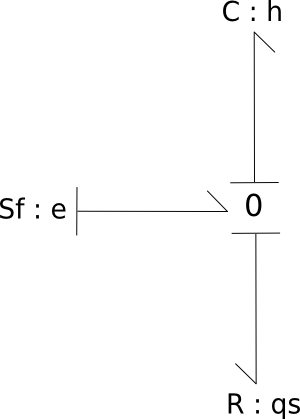
\includegraphics[scale=0.35]{tanque.png}
\end{figure}
\newpage

\section{Ejercicio 5}
Aquí introduciré el concepto de \emph{interés compuesto}. El cálculo del interés compuesto viene dado
por la siguiente ecuación:

\begin{equation*}
    {dA \over dt} = \lim_{\Delta t \rightarrow 0} { {\Delta A} \over {\Delta t} } = r A
\end{equation*}

donde:

\begin{itemize}
    \item $A(t)$
    \begin{itemize}
        \item Cantidad de dinero en una cuenta de ahorros en el instante t en años.
    \end{itemize}
    \item $r$
    \begin{itemize}
        \item Tasa de interés anual donde $0 \leq r \leq 1$.
    \end{itemize}
\end{itemize}

Básicamente el interés compuesto hace que los intereses periódicos de una inversión se reinviertan
en esa misma inversión periodo tras periodo. Esto se ve reflejado muy bien en la ecuación anterior.
\end{document}
